
\begin{figure}[htp]
\FIGURE
{\includegraphics[width=0.8\textwidth,height=\textheight,keepaspectratio]{./Figures/TA_Penetration.png}}
{LATENT PENETRATION\label{fig:latentpen}}
{Shows TripAdvisor's Penetration (left y-axis) across major US cities over time. The rank order of market penetration changes; Dallas surpasses Chicago and New York. Google Trends Index (right y-axis) documents the Google search results for "TripAdvisor."}
\end{figure}
\clearpage

\begin{figure}[htp]
\FIGURE
{\includegraphics[width=0.8\textwidth,height=\textheight,keepaspectratio]{./Figures/Smoothed_Qual_18987_v2.png}}
{LATENT QUALITY: Embassy Suites (Memphis, TN) \label{fig:latentqual}}
{Comparing this hotel's raw ratings and latent quality as measured by  Hotels.com,  Expedia,  and  pooled  OTA  ratings.  The raw  ratings  are  noisy  while the latent quality trends are smooth.}
\end{figure}
\clearpage

%%%% broken code: not compatible with INFORMS
% \begin{figure}[htp]
% \caption{EXAMPLES OF ESTIMATED LATENT MEASURES}
% % \label{fig:latent_graphs}
%      \centering
%      \begin{subfigure}
%          \centering
%          \includegraphics[width=0.5\textwidth,height=\textheight,keepaspectratio]{./Figures/TA_Penetration.png}
        
%         {(a) LATENT PENETRATION}
%          \label{fig:latentpen}
%      \end{subfigure}
     
%      \begin{subfigure}
%          \centering
%          \includegraphics[width=0.5\textwidth,height=\textheight,keepaspectratio]{./Figures/Smoothed_Qual_18987_v2.png}
         
%         {(b) LATENT QUALITY: Embassy Suites (Memphis, TN)}
%          \label{fig:latentqual}
%      \end{subfigure}
        
% \begin{flushleft}
% \small
% \textit{Note}. (a) Shows TripAdvisor's Penetration (left y-axis) across major US cities over time. The rank order of market penetration changes; Dallas surpasses Chicago and New York. Google Trends Index (right y-axis) documents the Google search results for "TripAdvisor." (b) Shows raw  ratings  are  noisy  while the latent quality trends are smooth.
% \end{flushleft}
% \end{figure}
% \clearpage

\begin{figure}[htp]
\FIGURE
{\includegraphics[width=0.8\textwidth,height=\textheight,keepaspectratio]{./Figures/OTA_Brand_v_Chain_v_PenetrationV2.png}}
{CHAIN ADVANTAGE BY TRIPADVISOR PENETRATION LEVEL\label{fig:modelfree}}
{Brand Quality Advantage (left y-axis) is the difference between the average quality of all chains' and average quality of all independents'. Average TripAdvisor penetration across all markets is plotted verses the right y-axis. Brand advantage decreasing as TripAdvisor penetration increases.}
\end{figure}
\clearpage

\begin{figure}[htp]
\FIGURE
{\includegraphics[width=0.8\textwidth,height=\textheight,keepaspectratio]{./Figures/LasVegasMarkets.png}}
{EXAMPLE OF LAS VEGAS MARKETS\label{fig:vegas}}
{Sam's Town and Skyline both belong to the Boulder Strip (as identified by HDBSCAN in pink) but belong to different TripAdvisor markets (as identified in blue). On TripAdvisor, they are ranked against hotels in their respective municipalities rather than against other hotels on the Boulder Strip.}
\end{figure}
\clearpage

\begin{figure}[htp]
\FIGURE
{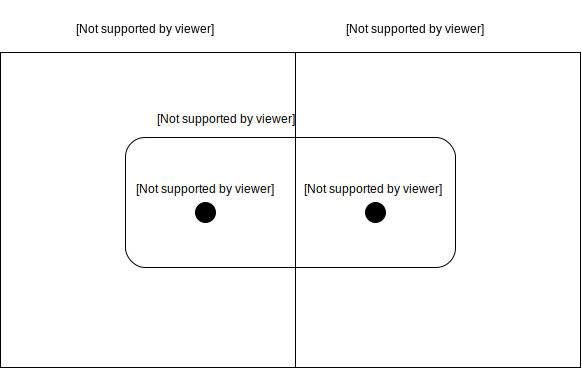
\includegraphics[width=0.8\textwidth,height=\textheight,keepaspectratio]{./Figures/Schematic.png}}
{SCHEMATIC REPRESENTATION OF EMPIRICAL TEST\label{fig:abmarkets}}
{}
\end{figure}
\clearpage

\begin{figure}[htp]
\FIGURE
{\includegraphics[width=0.8\textwidth,height=\textheight,keepaspectratio]{./Figures/clusters.png}}
{HDBSCAN AND K-MEANS COMPARISON\label{fig:cluster}}
{HDBSCAN is able to detect the visually intuitive clusters while k-means, a common clustering algorithm, struggles.}
\end{figure}
\clearpage

\begin{figure}[htp]
\FIGURE
{\includegraphics[width=0.8\textwidth,height=\textheight,keepaspectratio]{./Figures/brand_coeff2.png}}
{EROSION OF BRAND QUALITY ADVANTAGE\label{fig:brandvspenetrate}}
{This graph plots brand advantage (x-axis) versus the ddvantage erosion effect (brand$\times$penetration effect, y-axis), the black (gray) dots are brands with statistically significant (insignificant) quality advantages. The region above (below) the dotted diagonal line represents brands that hold a quality advantage (disadvantage) in a market with median levels of peak TripAdvisor penetration. The dots' diameters represent the relative total room capacities of brands.}
\end{figure}
\clearpage


